% Tikz File 'mytikz.tex'
\documentclass{standalone}
\usepackage{tikz}
%\usetikzlibrary{...}
\begin{document}
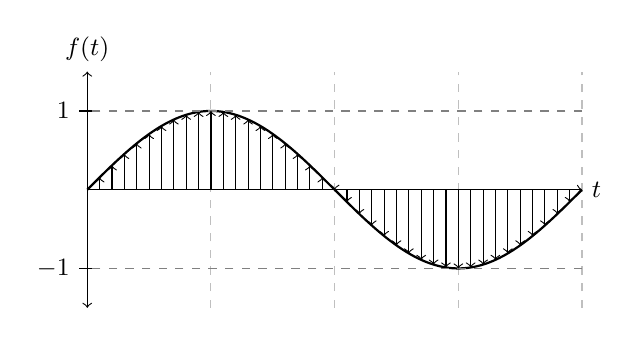
\begin{tikzpicture}
  % Add grid
  % \draw[gray!50, dashed, step=pi/4] (0,-1.5) grid (2*pi,1.5);
  \draw[gray!50, dashed, step=pi/2] (0,-1.5) grid (2*pi,1.5);

  % Draw the sine function
  \draw[domain=0:2*pi, samples=100, smooth, variable=\x, thick] plot ({\x}, {sin(\x r)});

  % Add axes
  \draw[->] (0,0) -- (2*pi,0) node[right] {\small $t$};
  \draw[<->] (0,-1.5) -- (0,1.5) node[above] {\small $f(t)$};

  \foreach \y in {-1, 1} {
      \draw (0.1,\y) -- (-0.1,\y) node[left] {\small $\y$};
      \draw [gray, dashed] (2*pi,\y) -- (0,\y);
    }

  \foreach \i in {0.05, 0.10, ..., 2.0} {
      \pgfmathsetmacro{\x}{\i * pi}
      \draw[->] (\x, 0) -- (\x, {sin(\x r)});
    }

\end{tikzpicture}
\end{document}


